\documentclass[11pt,letterpaper]{article}
\usepackage{color}
\usepackage{amsmath}
\usepackage{charter}
\usepackage[bitstream-charter]{mathdesign}
\usepackage[T1]{fontenc}
\usepackage{graphicx}
\usepackage{caption}
\usepackage{url}
\usepackage[top=1in, bottom=1in, left=1in, right=1in]{geometry}
\usepackage{setspace}
\usepackage[utf8]{inputenc}
 
\linespread{1.9}
\setlength\parindent{0.0in}
\setlength\parskip{0.2in}

\usepackage{fancyhdr}
\usepackage[super,comma]{natbib}
\pagestyle{fancy}
\fancyhf{} % clear all header and footer fields
\fancyfoot[R]{\footnotesize \thepage}
\renewcommand\headrulewidth{0pt}
\newcommand\caret{\mathbin{\char`\^}}

\newcommand{\comment}[1]{\colorbox[rgb]{0.988,0.914,0.31}{#1}}
\usepackage[resetlabels]{multibib}
\newcites{main}{References}
\newcites{supp}{Supplemental references}
\setbiblabelwidth{29}

\begin{document}

{\bf \LARGE Supplementary notes: qTrace algorithmic details}

In addition to the outline of the qTrace algorithm provided in the main text,
a detailed explanation of label definitions including variable labels and an 
exemplary comparison of the {\em fixed peak count} and the 
{\em isotope envelope fitting} modes follow.

% {\bf \large Label definition}
% moved to main text


{\bf \large Variable labels}

% The input of qTrace is formed by MS1 full scans and a list of target peptides.
% The label can be specified freely using the following notation:
% 
% ( <scope> (<isotope> <element> <labeling efficiency>)+ )+
% 
% \begin{description}
% \item [\tt 15N]
% $^{15}$N in all amino acids
% \item [\tt RK 13C 15N]
% $^{15}$N in all amino acids
% \end{description}

In the following example, the effect of defining a variable label is shown.
A fixed number of 3 required peaks per isotope envelope has been chosen, and the 
label has been defined as {\tt RP* 13C}, indicating a $^{13}$C label in every arginine 
residue, and also variably in every proline residue, as indicated 
by the star symbol.

\begin{figure}[h]
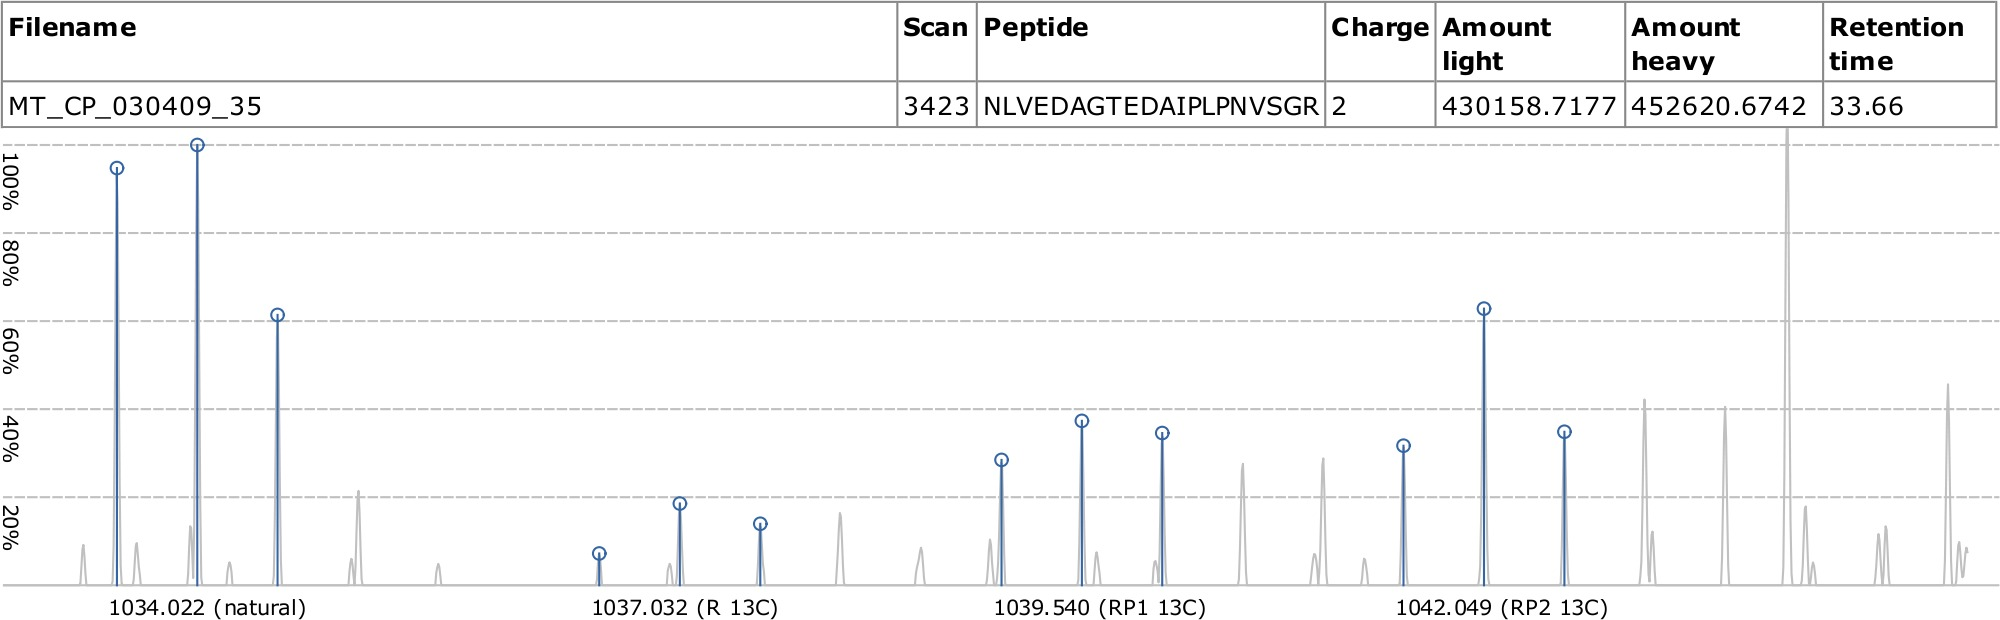
\includegraphics[width=\textwidth]{craft/NLVEDAGTEDAIPLPNVSGR-3-peaks.jpg}
\end{figure}

The quantified peptide NLVEDAGTEDAIPLPNVSGR contains 2 proline residues, thus
resulting in 2 additional heavy isotope envelopes for 1 or 2 labeled proline 
residues respectively.
It can be seen from the example figure that the heavy sister peptide amount 
would be dramatically underestimated if the additional heavy proline isotope 
envelopes would not have been taken into account.

{\bf \large Isotope envelope fitting}

As an alternative to the {\em fixed peak count} mode, qTrace provides the
{\em isotope envelope fitting} mode, which obviates the need to define a
somewhat arbitrary number of isotope peaks per isotope envelope. In this mode,
the actual number of isotope peaks depends on the theoretical isotope envelope
of a target peptide and is defined indirectly by the relative peak height in 
the theoretical isotope envelope. The following figure shows an example sister 
peptide pair as quantified with a fixed peak count of 3.

\begin{figure}[h]
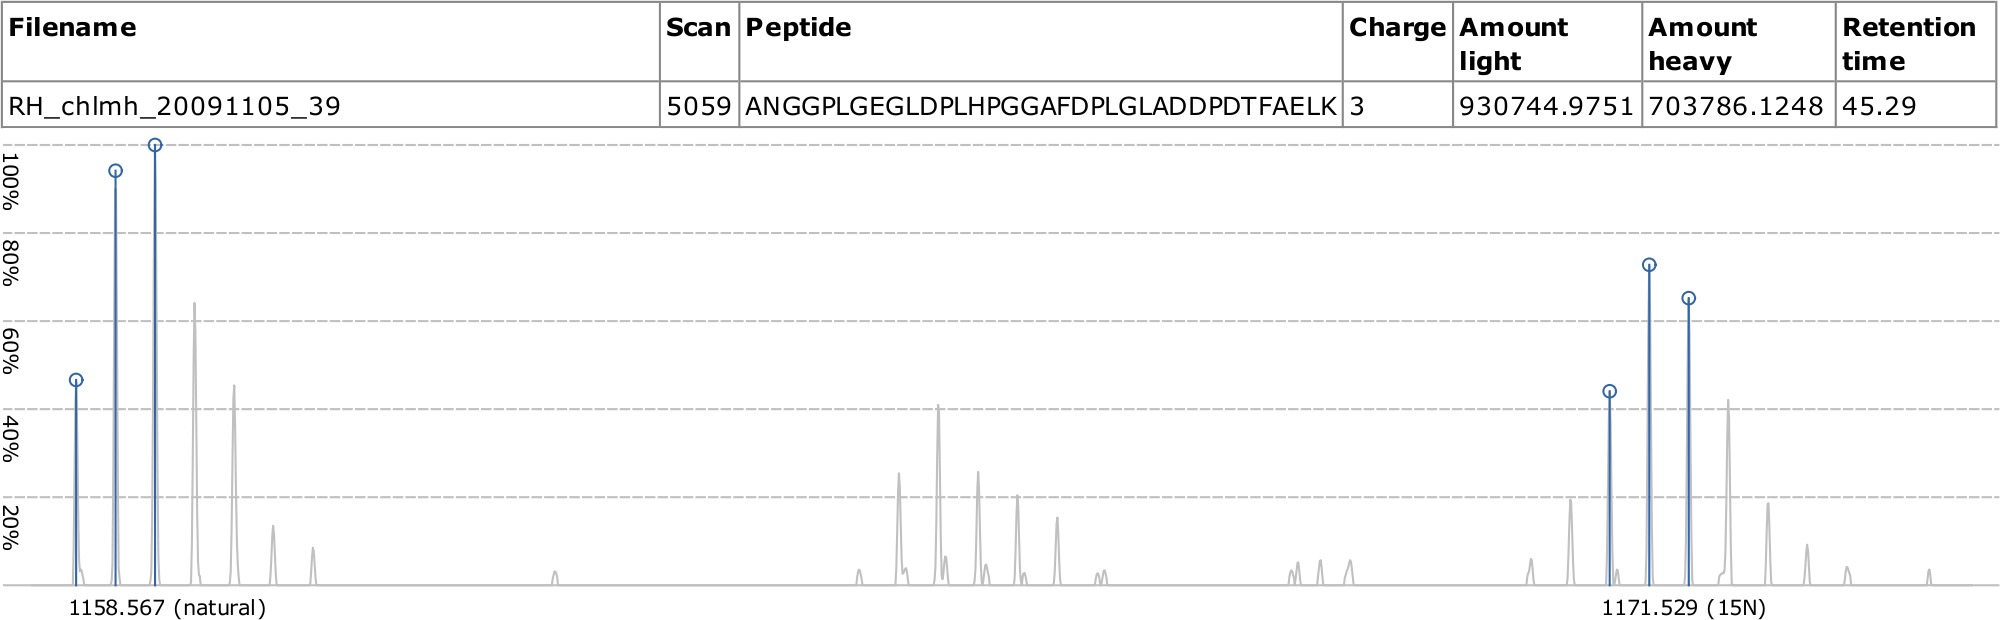
\includegraphics[width=\textwidth]{craft/5059-fixed.jpg}
% ratio is 1.322482701
\end{figure}

It can be seen that some peaks are not taken into consideration, although they
obviously stem from the same peptide and should contribute to the total amount.
For the following figure, isotope envelope fitting has been used with a 
{\em required peak abundance} of 40\% and a {\em considered peak abundance}
of 1\%. The amounts are estimated by determining the area under the fitted
theoretical isotope envelope, indicated by grey shading.

\begin{figure}[h]
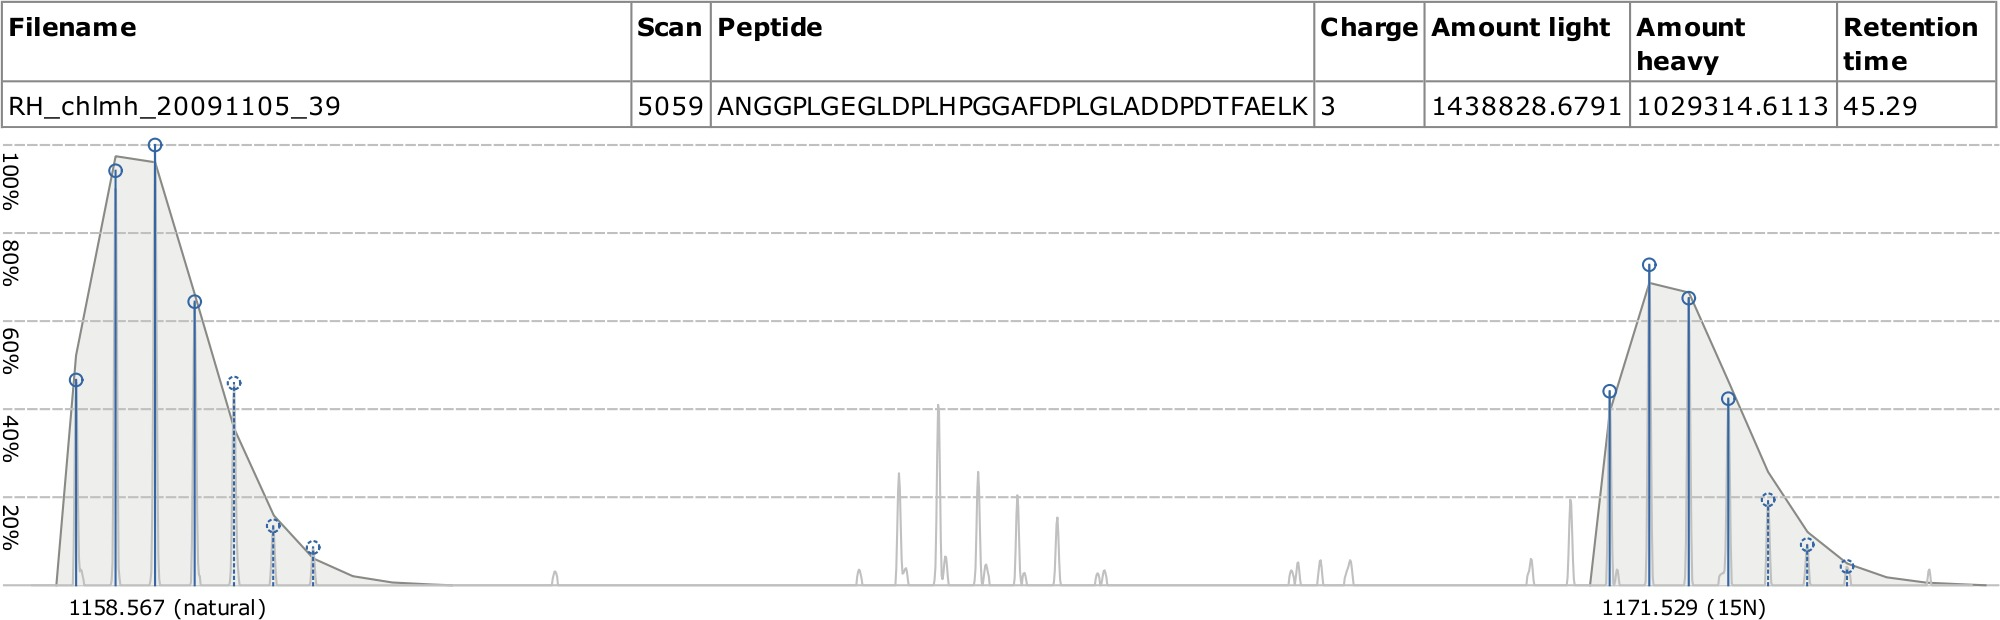
\includegraphics[width=\textwidth]{craft/5059-fitting-1000.jpg}
% ratio is 1.397851214
\end{figure}

Although the fitted isotope envelopes seem to match quite well, two additional
peaks are visible on the left hand side of the heavy isotope envelope, 
indicating that the $^{15}$N label was not completely incorporated and a small
amount of $^{14}$N atoms is still present in the heavy sample. Specifying
a labeling efficiency of 99.4\% leads to a slightly shifted isotope envelope
which captures the aforementioned two peaks, as demonstrated in the following 
figure.

\begin{figure}[h]
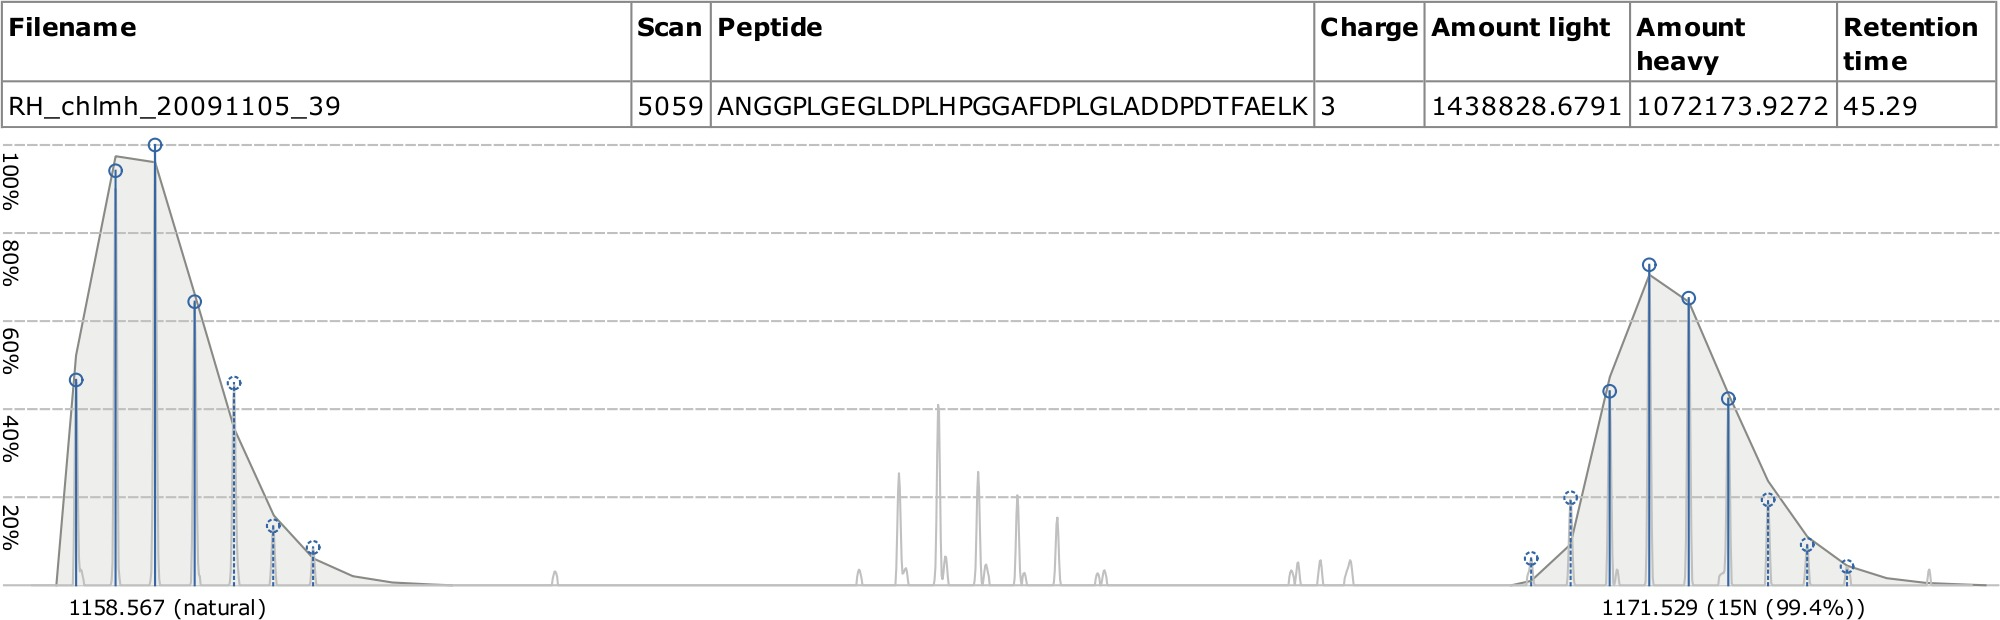
\includegraphics[width=\textwidth]{craft/5059-fitting-0994.jpg}
% ratio is 1.341973203
\end{figure}

\clearpage  

{\bf \LARGE Supplementary Figure S1: A Proteomatic pipeline for protein 
identification and quantitation explained in detail}

%%%%%%%%%%%%%%%%%%%%%%%%%%%%%%%%%%%%%%%%%%%%%%%%%%%%%%%%%%%%%%%%%%%%%%
%%%%%%%%%%%%%%%%%%%%%%%%%%%%%%%%%%%%%%%%%%%%%%%%%%%%%%%%%%%%%%%%%%%%%%
%%%%%%%%%%%%%%%%%%%%%%%%%%%%%%%%%%%%%%%%%%%%%%%%%%%%%%%%%%%%%%%%%%%%%%
%%%%%%%%%%%%%%%%%%%%%%%%%%%%%%%%%%%%%%%%%%%%%%%%%%%%%%%%%%%%%%%%%%%%%%
%%%%%%%%%%%%%%%%%%%%%%%%%%%%%%%%%%%%%%%%%%%%%%%%%%%%%%%%%%%%%%%%%%%%%%
%%%%%%%%%%%%%%%%%%%%%%%%%%%%%%%%%%%%%%%%%%%%%%%%%%%%%%%%%%%%%%%%%%%%%%
% ATTENTION ATTENTION: FIXED REFERENCE TO FIGURE 3 !!!!!!!!!!!!!!!!
%%%%%%%%%%%%%%%%%%%%%%%%%%%%%%%%%%%%%%%%%%%%%%%%%%%%%%%%%%%%%%%%%%%%%%
%%%%%%%%%%%%%%%%%%%%%%%%%%%%%%%%%%%%%%%%%%%%%%%%%%%%%%%%%%%%%%%%%%%%%%
%%%%%%%%%%%%%%%%%%%%%%%%%%%%%%%%%%%%%%%%%%%%%%%%%%%%%%%%%%%%%%%%%%%%%%
%%%%%%%%%%%%%%%%%%%%%%%%%%%%%%%%%%%%%%%%%%%%%%%%%%%%%%%%%%%%%%%%%%%%%%
%%%%%%%%%%%%%%%%%%%%%%%%%%%%%%%%%%%%%%%%%%%%%%%%%%%%%%%%%%%%%%%%%%%%%%
%%%%%%%%%%%%%%%%%%%%%%%%%%%%%%%%%%%%%%%%%%%%%%%%%%%%%%%%%%%%%%%%%%%%%%
In order to clarify the processing pipeline depicted in Fig.~3, 
a detailed description of the individual steps follows, in topological order
of the processing steps.
Please note that the workflow can be easily changed by re-arranging arrows, 
adding new processing steps, or adjusting the parameters in the right hand pane
of the window.
The pipeline was set up for a mass spectrometric experiment that dealt with a
sample containing differentially labeled $^{15}$N/$^{14}$N mixed iron-sufficient
and -deficient {\em C. reinhardtii} chloroplasts that were separated by 
one-dimensional SDS-PAGE. Individual protein bands were excised, digested with 
trypsin and analyzed by Nano-LC-coupled mass spectrometry as 
described\citesupp{terashima_characterizing_2010-1}.

\begin{figure}[h]
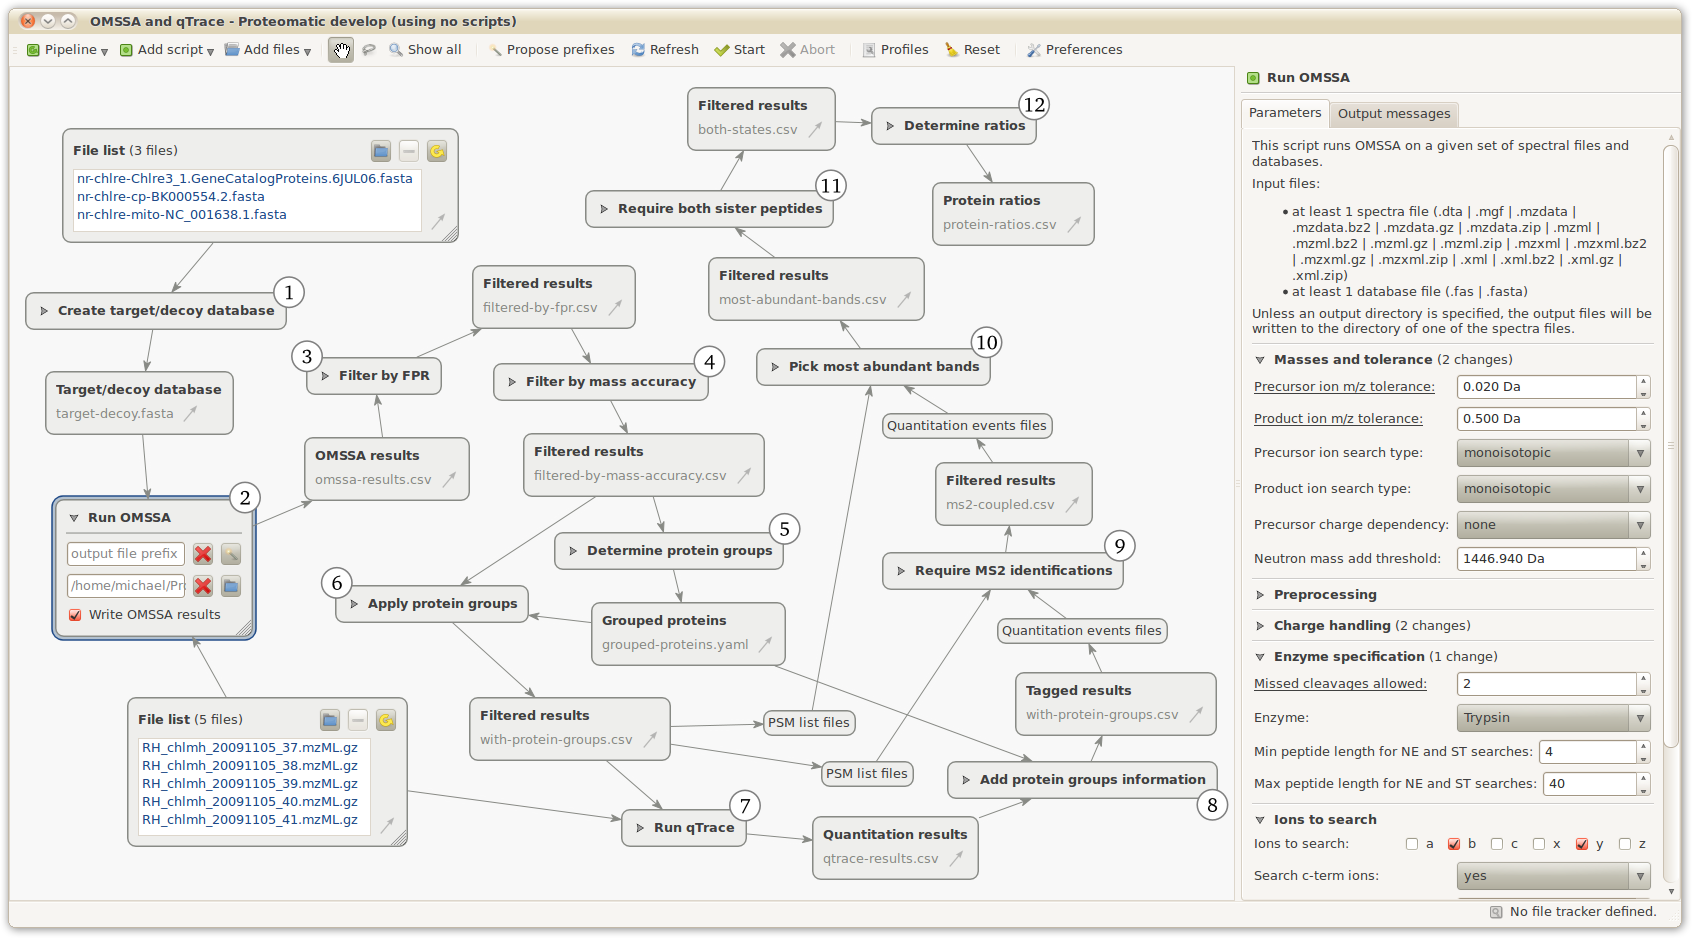
\includegraphics[width=\textwidth]{proteomatic-new-figure-annotated.jpg}
\end{figure}

\begin{enumerate}

\item {\bf Create target/decoy database.} 
A target/decoy database is assembled from the {\em C. reinhardtii} 
gene models deduced from nuclear, chloroplast, and mitochondrial genome 
databases\citesupp{merchant_chlamydomonas_2007}, with decoys being created by 
reversing the input sequences.

\item {\bf Run OMSSA.} 
OMSSA is used to perform an {\em in silico} tryptical digestion of the input 
target/decoy protein database and match the resulting tryptic peptides to the 
input fragmentation scans.

\item {\bf Filter by FPR.}
The resulting {\em true positive} (targets) and {\em false positive} (decoys) 
peptide/spectral matches (PSM) are sorted by score and an adaptive score 
threshold is determined in such a way that the estimated FPR is not higher 
than 1\%, according to the formula 
$FPR = \frac{2 \cdot decoys}{targets + decoys}$. 
Matches to peptides from decoy proteins are discarded.

\item {\bf Filter by mass accuracy.}
The remaining PSM are filtered by a 5 ppm precursor mass accuracy filter,
compensating for the fact that OMSSA only handles absolute mass tolerances.

\item {\bf Determine protein groups.}
Because peptides that appear in multiple proteins cannot be unambiguously 
assigned, the affected proteins are grouped as far as possible in this 
step\citesupp{nesvizhskii_interpretation_2005}: two proteins A and B are joined 
into a protein group if the identified peptides of protein A are a subset of 
the identified peptides of protein B. This way, protein families sharing equal 
peptides may be identified and later quantified as a protein group.

\item {\bf Apply protein groups.}
The protein groups are applied to the filtered OMSSA results by replacing the
protein entry of every PSM by the appropriate protein group.

%%%%%%%%%%%%%%%%%%%%%%%%%%%%%%%%%%%%%%%%%%%%%%%%%%%%%%%%%%%%%%%%%%%%%%
%%%%%%%%%%%%%%%%%%%%%%%%%%%%%%%%%%%%%%%%%%%%%%%%%%%%%%%%%%%%%%%%%%%%%%
%%%%%%%%%%%%%%%%%%%%%%%%%%%%%%%%%%%%%%%%%%%%%%%%%%%%%%%%%%%%%%%%%%%%%%
%%%%%%%%%%%%%%%%%%%%%%%%%%%%%%%%%%%%%%%%%%%%%%%%%%%%%%%%%%%%%%%%%%%%%%
%%%%%%%%%%%%%%%%%%%%%%%%%%%%%%%%%%%%%%%%%%%%%%%%%%%%%%%%%%%%%%%%%%%%%%
%%%%%%%%%%%%%%%%%%%%%%%%%%%%%%%%%%%%%%%%%%%%%%%%%%%%%%%%%%%%%%%%%%%%%%
% ATTENTION ATTENTION: FIXED REFERENCE TO FIGURE 4 !!!!!!!!!!!!!!!!
%%%%%%%%%%%%%%%%%%%%%%%%%%%%%%%%%%%%%%%%%%%%%%%%%%%%%%%%%%%%%%%%%%%%%%
%%%%%%%%%%%%%%%%%%%%%%%%%%%%%%%%%%%%%%%%%%%%%%%%%%%%%%%%%%%%%%%%%%%%%%
%%%%%%%%%%%%%%%%%%%%%%%%%%%%%%%%%%%%%%%%%%%%%%%%%%%%%%%%%%%%%%%%%%%%%%
%%%%%%%%%%%%%%%%%%%%%%%%%%%%%%%%%%%%%%%%%%%%%%%%%%%%%%%%%%%%%%%%%%%%%%
%%%%%%%%%%%%%%%%%%%%%%%%%%%%%%%%%%%%%%%%%%%%%%%%%%%%%%%%%%%%%%%%%%%%%%
%%%%%%%%%%%%%%%%%%%%%%%%%%%%%%%%%%%%%%%%%%%%%%%%%%%%%%%%%%%%%%%%%%%%%%
\item {\bf Run qTrace.}
The peptides identified by OMSSA and the spectral files are passed to qTrace,
which searches for unlabeled and $^{15}$N labeled sister peptides in MS1 full 
scans, as depicted in Fig.~4. At this time, the resulting 
quantitation events (QE) are available on the peptide level only.

\item {\bf Add protein groups information.}
The quantitation events are shifted to the protein level by adding the
appropriate protein group for every quantified peptide, discarding quantitation
events from peptides that appear in multiple protein groups.

\item {\bf Require MS2 identifications.}
In order to increase the confidence that the observed isotope envelopes in the 
MS1 full scans are really the target peptides, an MS2 fragment scan 
identification is required within a retention time difference of no more than 1 
minute. The necessary information is taken from the final filtered OMSSA 
result file. 

{\em Note:} The input boxes labeled {\em PSM list files} and {\em Quantitation 
events files} are necessary in the pipeline to resolve filename extension
ambiguities. Whenever possible, Proteomatic determines the correct files for 
an input file group by their filename extension (e. g. {\em Run OMSSA} requires
two input file groups {\em spectra} and {\em protein databases}, and input files
can be distinguished automatically because the filename extensions differ:
{\tt .fasta} for protein databases, {\tt .mzML} etc. for spectra files).
However, because both {\em Run OMSSA} and {\em Run qTrace} use the CSV format
for output files, the user must tell Proteomatic which files should be assigned 
to which input group by connecting the appropriate files to the input file 
group boxes instead of the script box.

\item {\bf Pick most abundant SDS-PAGE bands.}
To further reduce the risk of falsely assigned quantitation events, the OMSSA
identification results are used to determine the SDS-PAGE band where a 
protein (or protein group) was most abundantly identified in, and only 
quantitation events from this band ($\pm 1$ band) are retained.

\item {\bf Require both sister peptides.}
As a final filtering step, all quantitation events in which only one of the two
sister peptides is observed are discarded.

\item {\bf Determine ratios.}
Until here, only abundances have been estimated for both light and heavy sister
peptides, and no ratios have been calculated yet. Following the observation that
peptides are generally visible in multiple subsequent MS1 full scans while they
elute from the HPLC, we group the quantitation events of any peptide by its
combination of charge state and SDS-PAGE band, thereby capturing the elution 
process of any peptide. For each of these groups, all light and 
heavy abundances are added and divided to yield a ratio per 
peptide/band/charge (PBC) combination. The final protein (or 
protein group) ratio is obtained from calculating the mean and standard 
deviation of the individual PBC combination ratios.

\end{enumerate}

\clearpage  

{\bf \LARGE Supplementary Figure S2: qTrace metabolic labeling demonstration}

In order to assess the performance of qTrace, isolated chloroplast proteins from 
{\em Chlamydomonas reinhardtii} cultures grown under iron-deficient and 
iron-sufficient conditions were mixed and subsequently separated
via SDS-PAGE. A selection of five consecutive SDS-PAGE bands known to contain 
light-harvesting proteins were excised and tryptically digested and the 
resulting peptides further separated by an HPLC which was coupled on-line to a 
Thermo Scientific LTQ Orbitrap mass spectrometer, measuring each band for one 
hour, yielding a total of $\sim11,500$ full scans and $\sim18,000$ 
fragmentation scans. 
OMSSA was used to identify a total of 2,754 distinct peptides at an estimated 
FPR of 1\% and at a precursor mass accuracy of 5 ppm. 
The identified 
peptides were subsequently passed to qTrace, which was used to search for the 
individual unlabeled and $^{15}$N labeled isotope envelopes in all full scans. 
The resulting quantitation events were further filtered as described in 
{\bf Supplementary Figure 1}. 
After adding protein information and determining protein ratios, we were able to 
quantify a total of 59 proteins or protein groups, including many light 
harvesting proteins.

\begin{figure}[h]
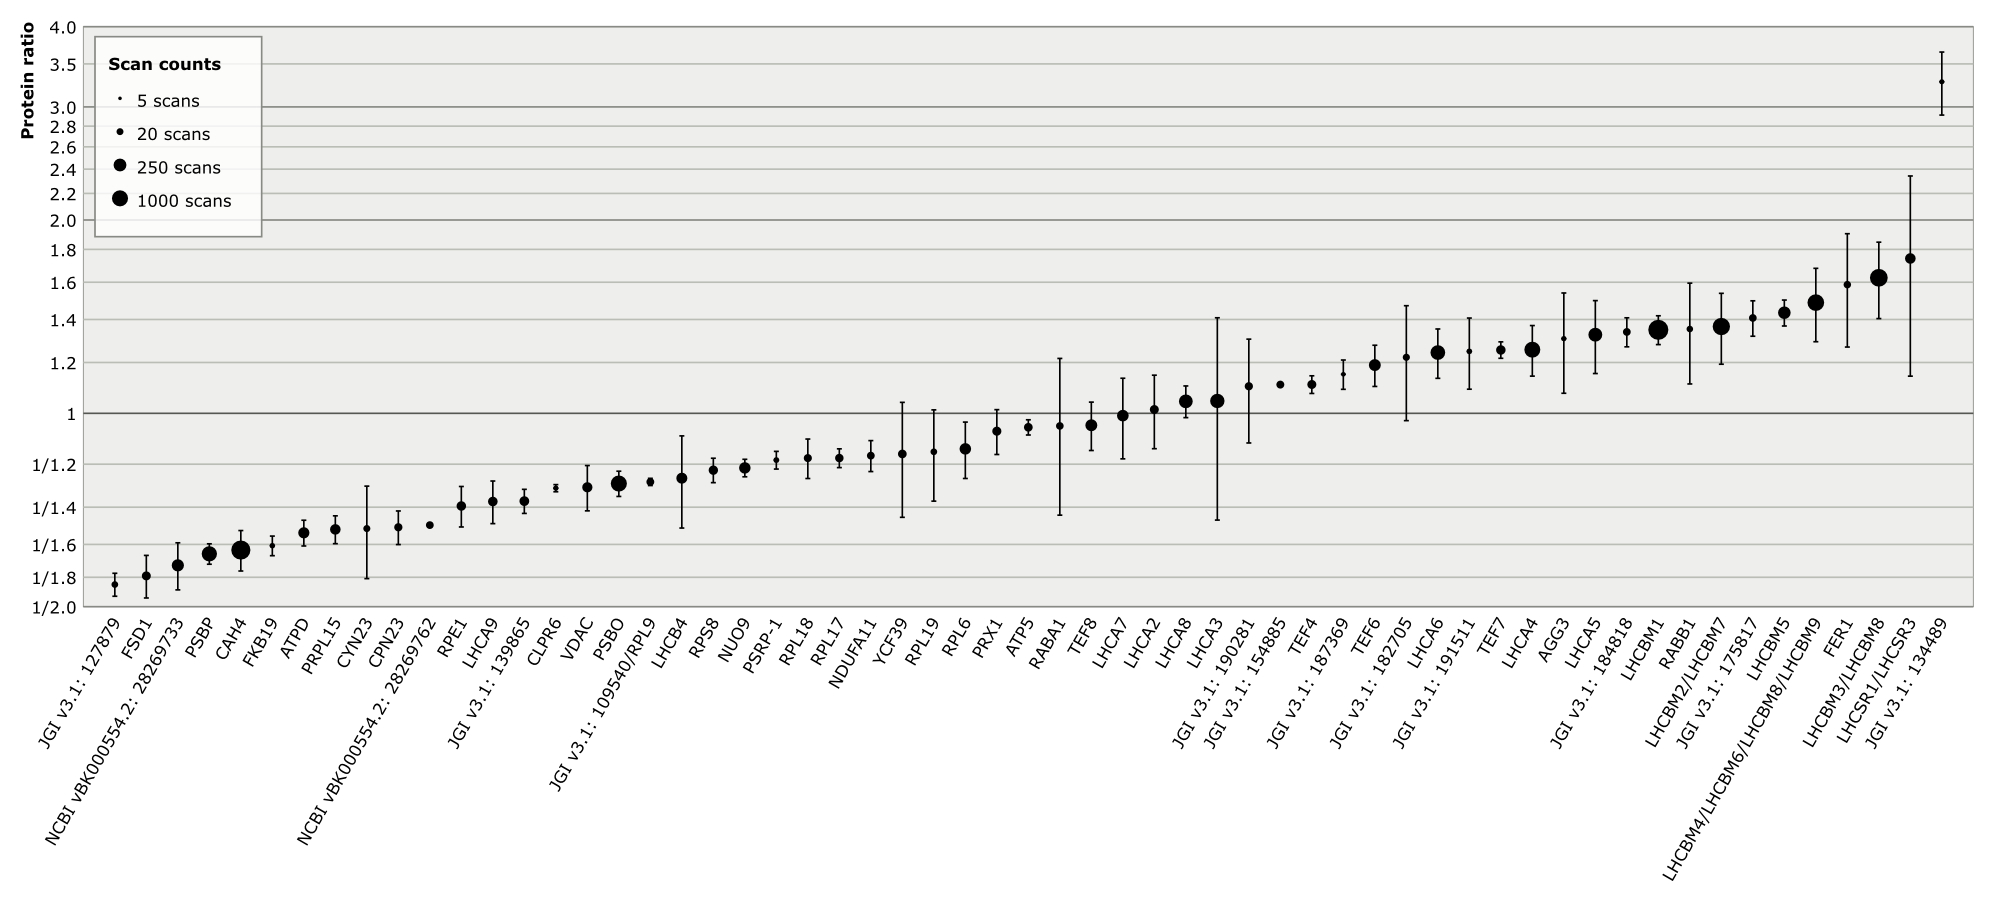
\includegraphics[width=\textwidth]{qtrace-diagram.jpg}
\end{figure}

\clearpage

{\bf \LARGE Supplementary Figure S3: qTrace performance assessment}

In order to assess the performance of qTrace, we have conducted a comparison 
between the well-established protein quantitation program 
MaxQuant\citesupp{cox_maxquant_2008-1} and qTrace. In the 
MaxQuant paper, a set of 24 measurements with three repeats was used for protein 
identification (using Mascot) and quantitation (using MaxQuant), leading to a 
total of $\sim4,100$ proteins quantified, $\sim3,800$ of which could be 
quantified with non-zero amounts in both light and heavy states. We performed 
the comparison based on these results only because quantitation results of 
zero or infinity must be considered less reliable due to the fact that one of 
the sister peptides might have escaped detection resulting from an unrecognized 
post-translational modification.

Using the same HeLa sample spectral files as in the MaxQuant paper (which are 
publicly available via Tranche) and the same IPI human protein database 
(version 3.48), we were able to quantify a total of $\sim2,200$ proteins (also 
with non-zero amounts for both light and heavy states). The fact that we could 
only identify 58\% of the proteins in comparison to the MaxQuant example likely 
results from the use of different search engines (Mascot vs. OMSSA) and, most 
of all, differences in the subsequent handling of peptide identification results. 
Regardless of the number of quantified proteins, the resulting protein ratios 
are consistent: 80\% of the results are within an acceptable difference range 
in which, for example, a MaxQuant ratio of 1.0 corresponds to a qTrace ratio of 
about 0.85 to 1.15, as shown in the comparison figure.

\begin{figure}[h]
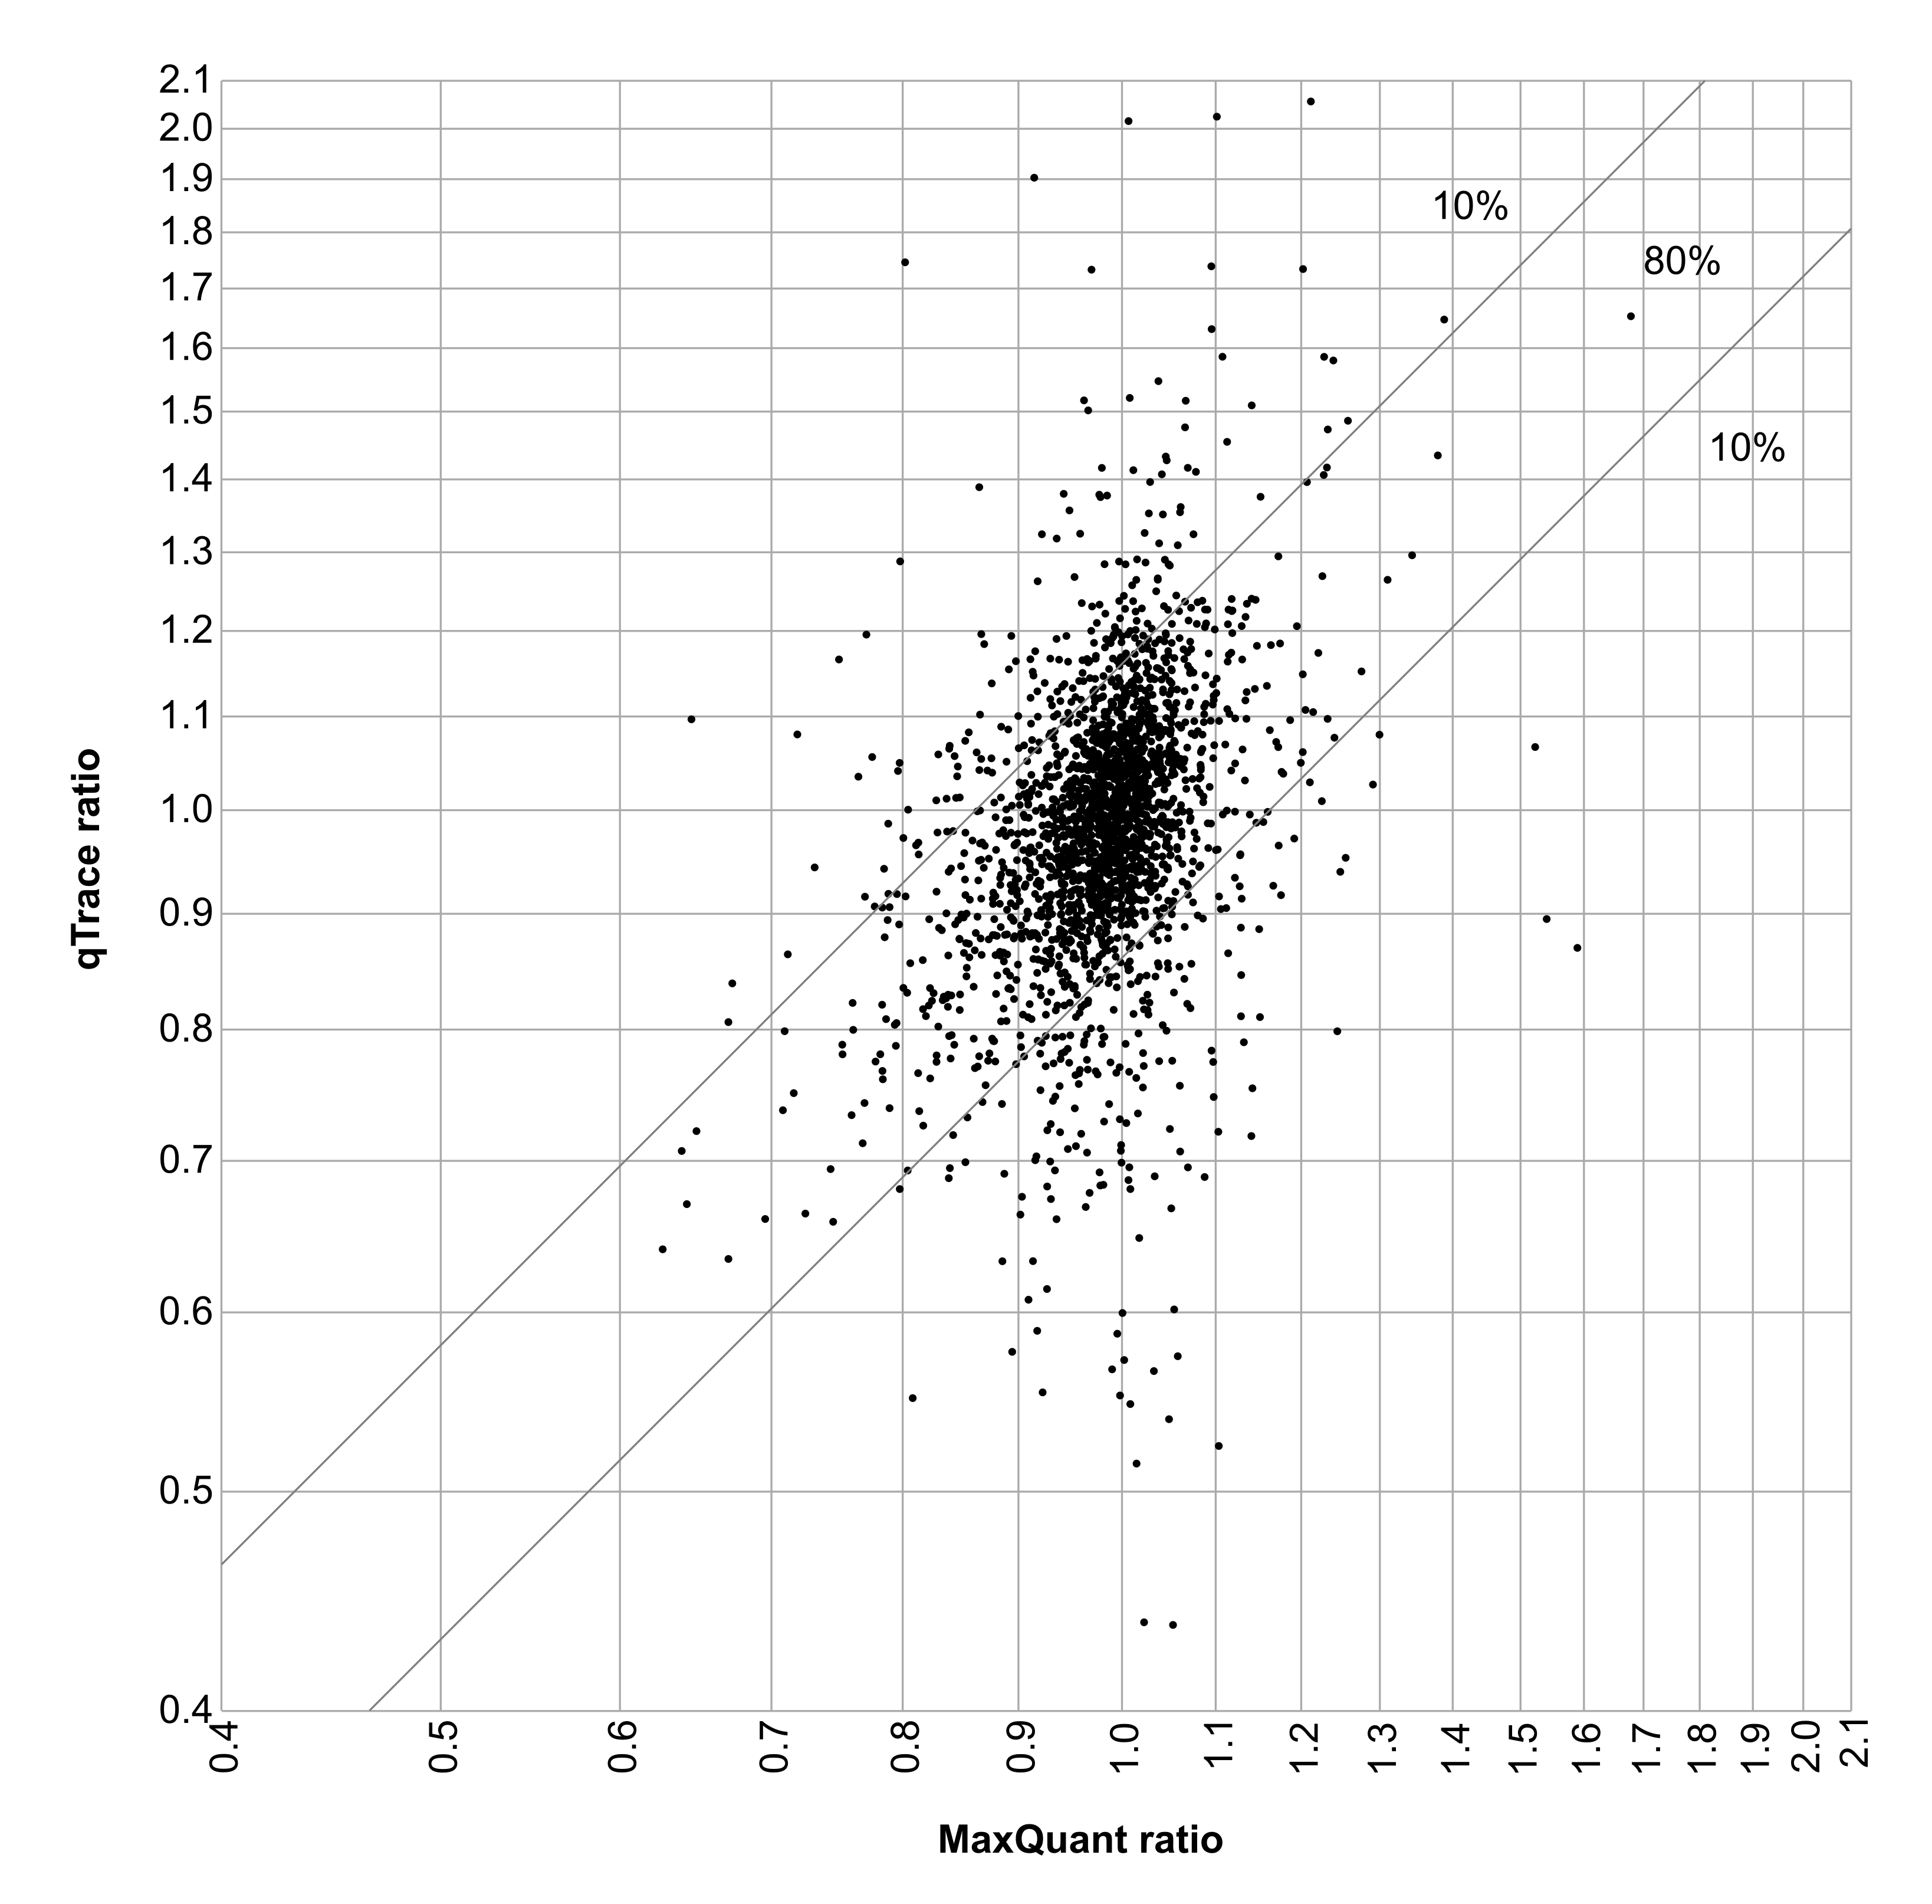
\includegraphics[width=\textwidth]{qtrace-maxquant.jpg}
\end{figure}

\clearpage

\begin{onehalfspacing}
\bibliographystylesupp{natbib}
\bibliographysupp{Proteomatic}
\end{onehalfspacing}

\end{document}
 
